\section{Funcionalidades}

No \calopsita{}, também por sua arquitetura de \textit{plugins}, as funcionalidades estão separadas em duas grandes partes: o núcleo e os \textit{plugins}. A primeira, contém apenas partes diretamente relacionadas com desenvolvimento ágil, no sentido mais amplo e irrestrito do termo -- sem interferência de metodologias, seus métodos e métricas. Essas partes, variáveis de cada projeto ou dependentes de metodologia, são deixadas para os \textit{plugins}, que dão ao sistema uma melhor adaptabilidade.

\subsection{Calopsita \textit{Core}}

As funcionalidades que fazem parte do núcleo do \calopsita{} consistem da criação e administração de usuários, projetos, cartões e iterações. Parece ser um núcleo minimal e essa é a intenção. Também faz parte do núcleo toda a infraestrutura necessária para a integração de um plugin ao sistema.

Essa seção se inicia com a proposta dos cartões, que é um tanto diferente e precisa ser explicada.

\subsubsection*{Cartões}

Diferente de outros sistemas com o mesmo propósito, o \calopsita{} não possui o conceito de histórias, mas apenas de cartões. Isso foi feito pensando em trazer maior grau de personalização para os usuários. Cada cartão pode ter subcartões e o que define a funcionalidade desse cartão é o conjunto de \textit{gadgets} que ele possui. 

A vantagem é que pode-se criar uma hierarquia, tão profunda quanto se desejar, para organizar tudo o que há para ser feito em um projeto. Isso também permite que o projeto possa ser visto no nível de detalhe mais apropriado pra cada envolvido no projeto, seja ele gerente, desenvolvedor ou cliente. 

\begin{figure}[H]
  \centering
  \fbox{
    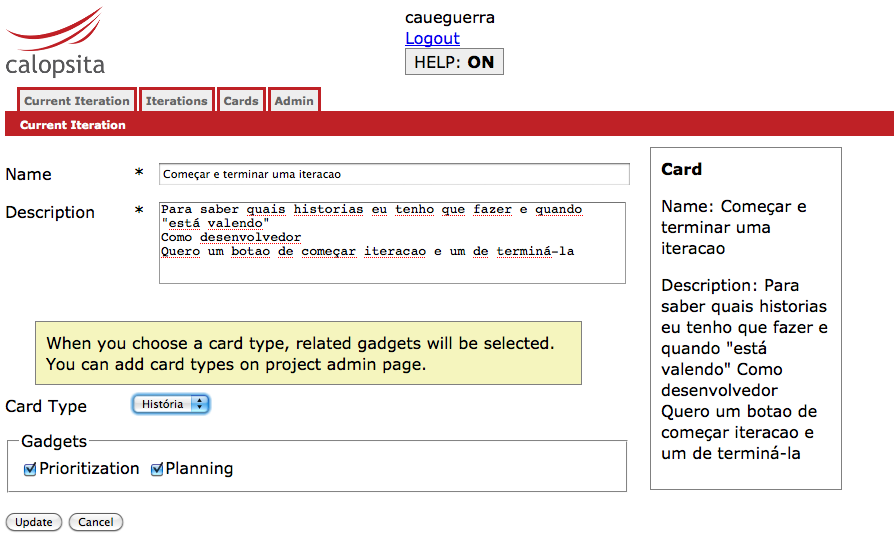
\includegraphics[width=110mm]{images/cartao.png}
  }
  \caption{Cartão}\label{figura:cartao}
\end{figure}

\begin{figure}[H]
  \centering
  \fbox{
    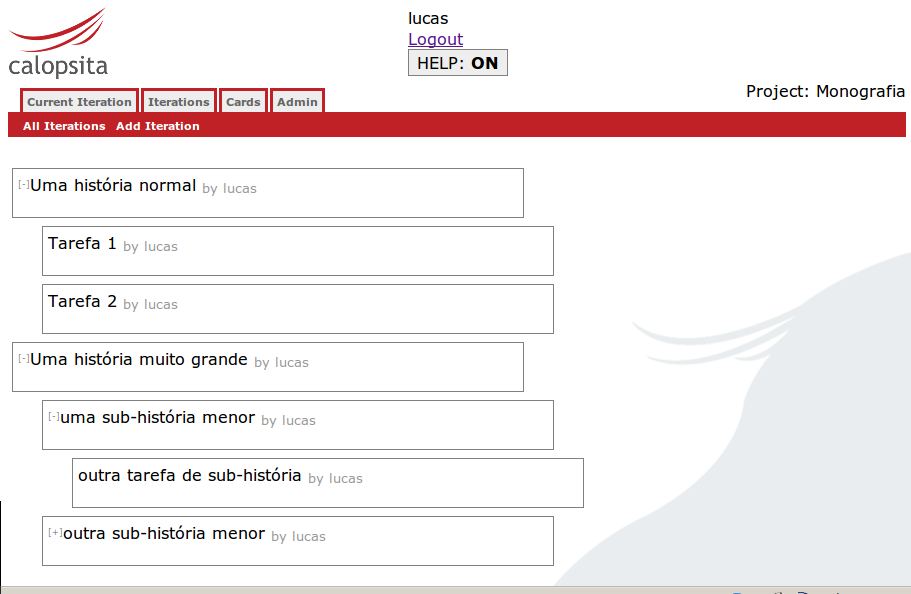
\includegraphics[width=110mm]{images/hierarquia-de-cartoes.png}
  }
  \caption{Cartões mostrados hierarquicamente}\label{figura:hierarquia}
\end{figure}

Já foi dito que usabilidade é uma questão importante para o \calopsita{}. Para determinar hierarquia de cartões foi cogitado utilizar cores diferentes para cartões de mesma grandeza. Preferiu-se, no entanto, usar a indentação mostrada na figura \ref{figura:hierarquia} para manter o sistema acessível para daltônicos.

\subsubsection*{Tipos de Cartões}

Um tipo de cartão é, para o \calopsita{}, um agrupamento de \textit{gadgets} que definem o comportamento de um determinado cartão. Perceba que a noção é puramente semântica, já que os \textit{gadgets} podem ser habilitados e desabilitados individualmente, por cartão.

No exemplo da figura \ref{figura:tipo_cartao}, abaixo, um tipo de cartão denominado "História" é criado e, a ele, são associados os \textit{gadgets} "Priorização" e "Planejamento". Deste momento em diante, sempre que um cartão do tipo "História" for criado, ele automaticamente marcará os \textit{gadgets} citados.

Dessa forma, a história criada aparecerá na tela de priorização e poderá ser adicionada a uma iteração -- por ser, respectivamente priorizável e planejável. 

\begin{figure}[H]
  \centering
  \fbox{
    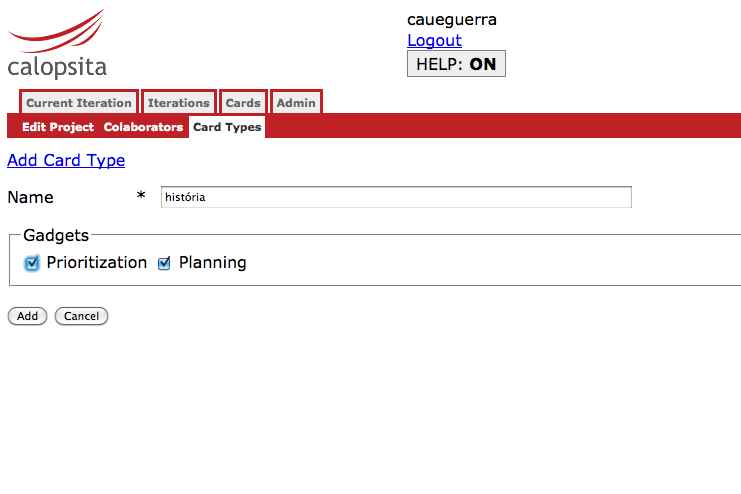
\includegraphics[width=110mm]{images/tipo_cartao.png}
  }
  \caption{Tipos de Cartões}\label{figura:tipo_cartao}
\end{figure}

\subsubsection*{Iterações}

Uma iteração é um ciclo de desenvolvimento ágil. No \calopsita{} é possível criar iterações, editar e removê-las. Na sua criação, é preciso estabelecer uma meta ou um tema da iteração e, além disso, pode-se escolher suas datas de início e fim.

Essas datas são opcionais já que ter ou não datas fechadas depende, exclusivamente, da metodologia adotada pelo time. Em \textit{Scrum}, por exemplo, as datas são pré-fixadas e imutáveis. Já em \textit{XP} preza-se mais pela flexibilidade e uma iteração pode começar ou acabar a qualquer momento.

Um time de \textit{Scrum} que use o \calopsita{} colocaria as datas de antemão e, no dia de início de uma iteração, veria-a começando automaticamente (no menu, "Iteração atual"). Já um time de \textit{XP} quando quisesse começar uma iteração, clicaria num ícone de \textit{Play} na iteração que deseja começar e num de \textit{Stop} para terminá-la. Se já houvesse datas e, por exemplo, a iteração fosse adiantada alguns dias, o intervalo de tempo entre o início e o fim se manteria -- ambas as datas seriam adiantadas. Veja o exemplo de ícone para iniciar uma iteração futura na figura \ref{figura:play}:

\begin{figure}[H]
  \centering
  \fbox{
    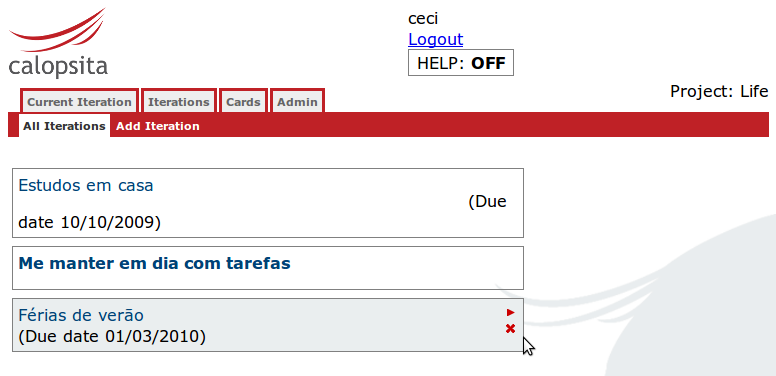
\includegraphics[width=110mm]{images/play_iteracao.png}
  }
  \caption{Adiantar o início de uma iteração}\label{figura:play}
\end{figure}

\subsubsection*{Usuários e projetos}

Por padrão, qualquer usuário pode se cadastrar no sistema. Basta preencher o cadastro com informações pessoais. Igualmente, qualquer usuário logado pode criar projetos.

Num projeto, é possível adicionar colaboradores. Para isso, há uma seção administrativa que permite adicionar um outro usuário ao projeto. Escolhe-se o usuário digitando o \textit{login} dele no campo de seleção ou escolhendo na lista de usuários disponíveis. Essa lista mostra apenas os usuário que ainda não fazem parte do projeto em questão.  

\subsubsection*{Registro de mudanças}

Está previsto para também fazer parte do núcleo do \calopsita{} uma funcionalidade de histórico de mudanças. Assim, será possível coletar informações para gerar gráficos e criar serviços que retornem as últimas modificações feitas, em formato RSS, para que os membros do projeto possam utilizar agregadores de notícias como o \textit{Google Reader} para acompanhar o andamento da iteração.

\subsection{Calopsita Plugins}

Como explicado anteriormente, o \calopsita{} possuí um núcleo com as funcionalidades essenciais e as demais serão fornecidas através de \textit{plugins}. Há, no \textit{backlog} do \calopsita{}, diversos plugins a serem implementados e que já viriam na instalação padrão do \calopsita{}. Segue abaixo uma breve descrição de cada um deles:

\begin{itemize}
	\item{Priorização: permite seja atribuída uma prioridade a um determinado cartão através de uma interface baseada em \textit{drag 'n' drop}. Esse plugin já está implementado;
	
	\begin{figure}[H]
	  \centering
	  \fbox{
	    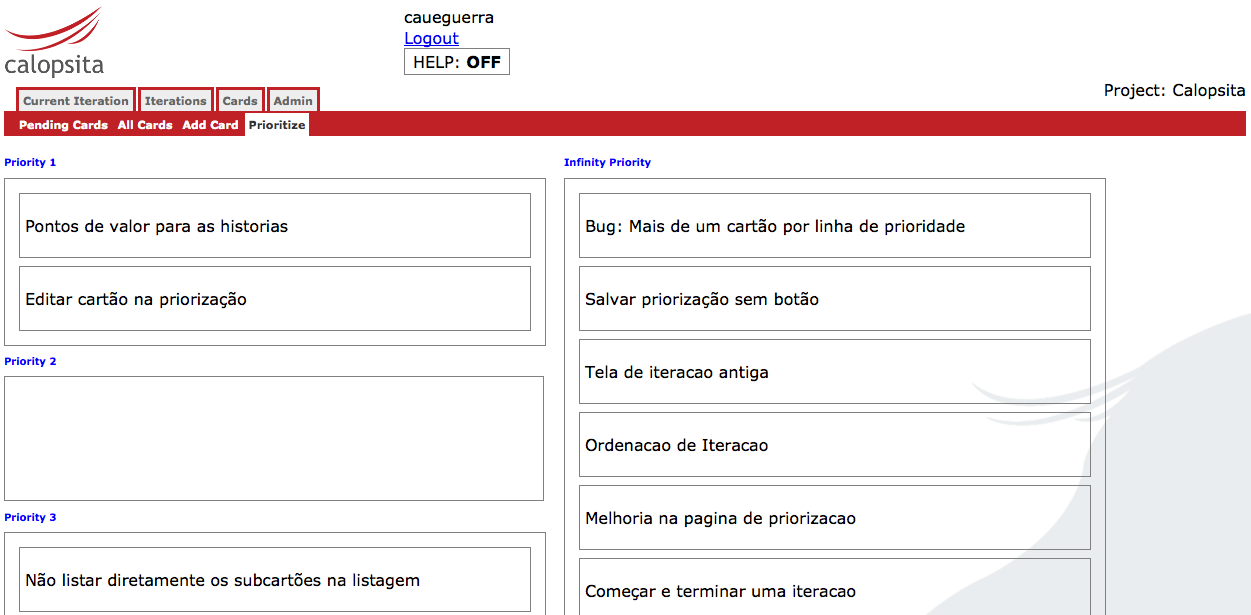
\includegraphics[width=110mm]{images/priorizacao.png}
	  }
	  \caption{Priorizacao}\label{figura:priorizacao}
	\end{figure}
	}
	\item{Planejamento: permite que cartões sejam adicionadas ou removidas de uma determinada iteração. Também baseado em \textit{drag 'n' drop} e já está implementado;
	
	\begin{figure}[H]
	  \centering
	  \fbox{
	    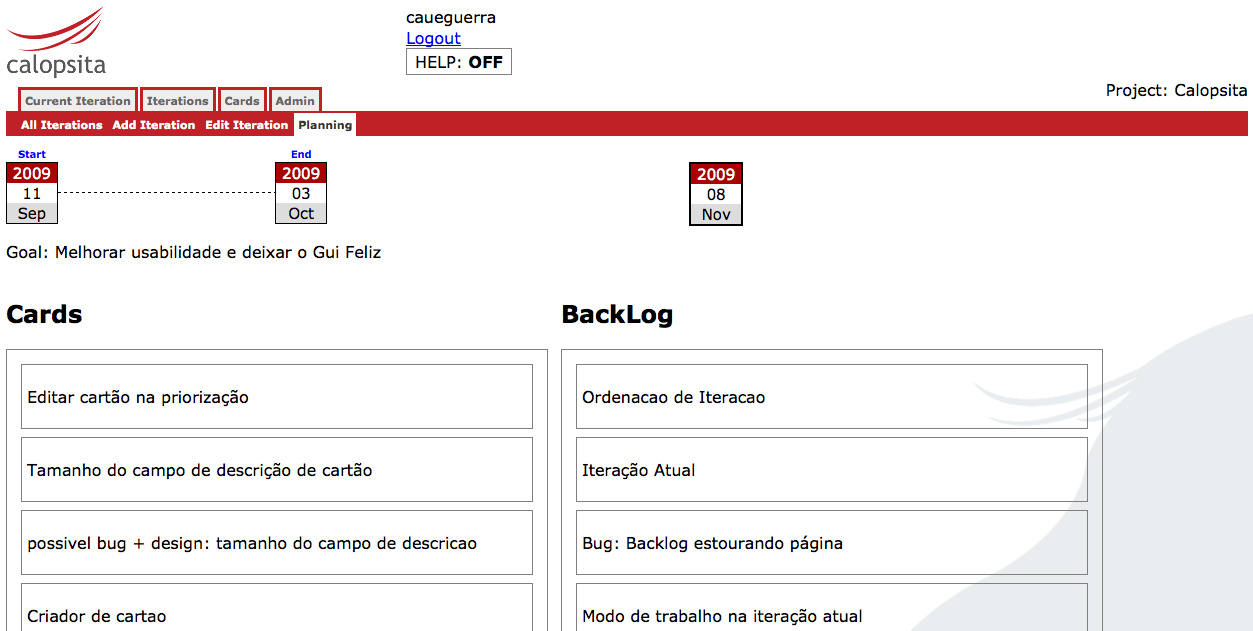
\includegraphics[width=110mm]{images/planejamento.png}
	  }
	  \caption{Planejamento}\label{figura:planejamento}
	\end{figure}
	}
	\item{Gráfico \textit{burn-up}: a idéia desse plugin é que uma nova página contendo o gráfico \textit{burn-up} de uma determinada iteração seja criada. Este gráfico possui uma linha horizontal, que representa a meta a ser atingida. Essa meta é baseada em alguma métrica da iteração: número de cartões, soma da dificuldade dos cartões, etc. Com o passar dos dias da iteração é marcada a evolução da métrica escolhida, de acordo com o número de cartões prontos;}
	\item{Gráfico \textit{burn-down}: a idéia desse plugin é que uma nova página contendo o gráfico \textit{burn-down} de uma determinada iteração sejá criada. Esse gráfico é parecido com o de \textit{burn-up}, mas a evolução se dá pela quantidade de uma métrica que ainda não está pronta. Geralmente possui uma linha decrescente que representa a velocidade estimada;}
	\item{Marcação de horas: esse plugin permitirá que a pessoa que trabalhou na conclusão de determinado cartão possa marcar o número de horas trabalhadas;}
	\item{Estimativas: possibilitará que um cartão tenha sua dificuldade estimada em pontos;}
	\item{Personas: criará uma área especial para a definição de personas. Essas personas poderão ser utilizadas mais facilmente na criação de novos cartões;}
	\item{Integração com GitHub: permitirá que comentários feitos no \textit{commit} do projeto no GitHub consigam mover cartões dentro de uma determinada iteração e mudar seu status.}
	\item{Modelos de metodologias: disponibilizar modelos pré-prontos com tipos de cartão, nomenclaturas e \textit{gadgets} habilitados que são específicos de uma metodologia. Por exemplo um modelo \textit{Scrum} teria os tipos de cartão ``História'', ``Épico'' e ``Tarefa'', a iteração se chamaria ``Sprint'' e teria uma ``Meta'', o \textit{Kanban} com as colunas ``Parado'', ``Em Andamento'', ``Em inspeção'' e ``Pronto'', etc.}
\end{itemize}
